%% LyX 2.1.1 created this file.  For more info, see http://www.lyx.org/.
%% Do not edit unless you really know what you are doing.
%\documentclass[letterpaper,twocol,amsmath,aps,jcp,preprintnumbers,groupaddress,nofootinbib,tightenlines]{revtex4-1}
%\usepackage[latin9]{inputenc}
%\usepackage{textcomp}

\documentclass[letterpaper,twocolumn,amsmath,amsfont,amssymb,english,aps,jcp,preprintnumbers,groupaddress,nofootinbib,tightenlines]{revtex4}

\usepackage{graphicx}


%\documentclass[aps,prb,letterpaper,twocolumn,nofootinbib,showkeys]{revtex4-1}
%\documentclass[aps,amssymb,prl,letterpaper,twocolumn,nofootinbib,showkeys]{revtex4-1}

%\usepackage[backend=bibtex]{biblatex}

%    backend=biber,
%    style=authoryear,
%    natbib=true,
%    sortlocale=en_US,
%    url=false,
%    doi=true,f
%    eprint=false
%]{biblatex}
%\usepackage{hyperref}


\newcommand{\mat}[1]{\boldsymbol{#1}}
\newcommand{\matT}[1]{\boldsymbol{#1}^\dagger}
\newcommand{\ot}{ {\scriptstyle \otimes}_{ \tau } }

%%\hypersetup{pdftitle={FreeON Project Report 1}}
%\hypersetup{pdfauthor={Matt Challacombe and Nicolas Bock}}
%\hypersetup{pdfsubject={A SpAMM Stabilized Newton Schulz Preconditioner: Fighting Error with Error}}

%\bibstyle{aipnum4-1}

\begin{document}

\title{On Stability of Newton Schulz Iterations in an Approximate Algebra}

\author{Matt Challacombe}
\email{matt.challacombe@freeon.org}
\homepage{http://www.freeon.org}
\affiliation{Theoretical Division, Los Alamos National Laboratory}

\author{Nicolas Bock}
\email{nicolasbock@freeon.org}
\homepage{http://www.freeon.org}
\affiliation{Theoretical Division, Los Alamos National Laboratory}

%\begin{abstract}
%Forward look
%\end{abstract}

\maketitle
\section{Introduction}

Decay principles, often very sparse but very ill-conditioned problems.

\subsection{Incomplete Schemes}

Incompleteness -> sparse approximations dense problems, uses conventional sparse infrastructure, second order errors in matrix multiplication.  
Often adhoc.

$\tilde{\mat{a}} = \mat{a}+ \delta \mat{a}$

$\tilde{\mat{a}} \cdot \tilde{\mat{b}} = \mat{a}\cdot\mat{b}+ \delta \mat{a} \cdot \mat{b} +  \mat{a} \cdot \delta \mat{b}
+  \delta \mat{a} \cdot \delta \mat{b}$

The variations do not express in the overal context of the product.  Because the error in the incomplete case is additive, the

 For example, 
$\mat{a}$ may be small, but $\delta \mat{a} \cdot \mat{b}$  large, leading extra work.  Also, 
once a truncation error is commited, it is encounted in all subsiquent steps; it becomes difficult to impossilbe to manage error flows of differing 
magnitude in complex maps. 


\subsection{On ``Variational'' and ``non-Variational'' Iteration}
Gradients lack convergence properties
Iteration without orig drives away from basis
NS has both.  Difference between scalar iteration, Higham page 92.

\subsection{\bf Methods that accumulate incompleteness  (purification, and Krylov subspace):} 

\subsection{\bf ``Variational'' Methods Stay Close to the Basis (LNV Gradients, RQI and Newton Shulz)} 
\subsection{Approximation with Incompleteness and Iteration: Corruption of the Eigen Basis}


\subsection{Approximate Algebras as {\bf \em N}-Body Problem}

\pagebreak


SpAMM is the recursive Cauchy-Schwarz occlusion product $\ot$ on matrix quadtrees

\begin{equation}
\mat{a}^i = \begin{bmatrix} \mat{a}^{i+1}_{00} & \mat{a}^{i+1}_{01} \\ \mat{a}^{i+1}_{10} & \mat{a}^{i+1}_{11} \end{bmatrix}
\end{equation}

\begin{widetext}
\begin{equation}
\mat{a}^{i} \ot \mat{b}^{i} = 
\left\{
        \begin{array}{ll}
                 \emptyset \quad \tt{if}\quad \lVert \mat{a}^i \rVert \lVert \mat{b}^i \rVert < \tau \\[0.2cm]
                 \mat{a} ^i \cdot \mat{b}^i \quad  \tt{if}(i=\tt{leaf}) \\[0.2cm]
\begin{bmatrix} \mat{a}^{i+1}_{00} \ot \mat{b}^{i+1}_{00} +\mat{a}^{i+1}_{01} \ot \mat{b}^{i+1}_{10} \; , \; &
                \mat{a}^{i+1}_{00} \ot \mat{b}^{i+1}_{01} +\mat{a}^{i+1}_{01} \ot \mat{b}^{i+1}_{11}  \\[0.2cm] 
                \mat{a}^{i+1}_{00} \ot \mat{b}^{i+1}_{01} +\mat{a}^{i+1}_{01} \ot \mat{b}^{i+1}_{11} \; , \; & 
                \mat{a}^{i+1}_{00} \ot \mat{b}^{i+1}_{01} +\mat{a}^{i+1}_{01} \ot \mat{b}^{i+1}_{11}   
\end{bmatrix}  \quad \tt{else}
                \end{array}
              \right.
\end{equation}
\end{widetext}







database orientation, Cauchy sch
Approximate Algebra, SpAMM Cauchy Schwarz occlusion, n-body approach to numerical linear algebra, first order errors in matrix multiplication.
Based on Cauchy Schwarz inequality.



error accumulation may be better than row-col
single programing model.  generacity.  communication optimality and strong scaling.

\subsection{Incomplete Algorithms and Aproximate Algebras} %%!what is spamm}

Incompleteness -> sparse approximations dense problems, uses conventional sparse infrastructure, second order errors in matrix multiplication.  
Often adhoc.

Philosophy: Don't know which elements to drop, because only make sense in context.  It is very difficult to incorporate this context in a dropping 
strategies. 

Approximate Algebra, SpAMM Cauchy Schwarz occlusion, n-body approach to numerical linear algebra, first order errors in matrix multiplication.
Based on Cauchy Schwarz inequality.

We show that this first order error in algebraic context follows the functional analysis, and enables the consideration {\em and seperate treatment} of
first order error flows in the analysis of complex maps. 

\begin{equation}
\mat{a} \ot \mat{b}=\mat{a}\cdot \mat{b} + \mat{\Delta}^{a\cdot b}_{\tau}
\end{equation}
where $\mat{\Delta}^{a \cdot b}_{\tau}$ is a deterministic first order variation cooresponding to the branch pattern set
by Cauchy-Schwarz culling, with length $\lVert \mat{\Delta}^{a \cdot b}_{\tau} \rVert \leq \tau \lVert \mat{a} \rVert  \lVert \mat{b} \rVert$.  

For a vector space $S$ with $\mat{a},\mat{b} \in S$, the opperator $\ot$ leads to a non-associative algebra with Lie bracket
\begin{equation}
\left[ \mat{a} , \mat{b} \right]_{\tau} =
\mat{a} \ot \mat{b}-\mat{b} \ot \mat{a} = \mat{\Delta}^{a\cdot b}_{\tau} -\mat{\Delta}^{b\cdot a}_{\tau} ,
\end{equation}
determined by the occlusion field.  Our challenge is to master the error flows of these occlusion fields under iteration, 
for ill-conditioned problems and with permisive values of $\tau$. 




\section{Newton Shulz Iteration}

\subsection{Idempotence }


\subsection{The Scaled Map}


\subsection{Alternative Formulations}






\pagebreak

\section{\bf  Mapping Error Flows}

\begin{equation}
\delta \mat{x}^{\rm{naiv}}_k =   \delta  \widetilde{ \mat{z}}_{k} \cdot \mat{s} \cdot \widetilde{\mat{z}}_{k} 
                           +  \widetilde{\mat{z}}_{k} \cdot \mat{s} \cdot \! \delta \widetilde{\mat{z}}_{k} 
\end{equation}



\begin{equation}
\delta \mat{x}^{\rm{dual}}_k =   \delta  \widetilde{ \mat{y}}_{k} \cdot \widehat{\mat{z}}_{k} 
                           +  \widetilde{\mat{y}}_{k} \cdot \delta \widetilde{\mat{z}}_{k} 
\end{equation}



\begin{eqnarray}
\widetilde{\mat{x}}_k &=& f \left[\widetilde{\mat{z}}_{k-1} , \widetilde{\mat{x}}_{k-1} \right] \\ 
&=&
\tt{m} \left[ \widetilde{\mat{x}}_{k-1}\right] \cdot \widetilde{\mat{z}}^\dagger_{k-1}  
\cdot \mat{s} \cdot \widetilde{\mat{z}}_{k-1} \cdot \tt{m}\left[ \widetilde{\mat{x}}_{k-1} \right] 
\nonumber
\end{eqnarray}

\begin{equation}
\delta \mat{x}_k = {f}_{\delta \mat{z}_{k-1}}  \, \lVert \delta \mat{z}_{k-1} \rVert 
                              +  {f}_{\delta \mat{x}_{k-1}}   \, \lVert \delta \mat{x}_{k-1} \rVert 
                                                                                      + {\cal{O}} \left(  \tau^2 \right)
\end{equation}

%                              +  {f}_{\delta \mat{z}_{k-1}, \delta \mat{x}_{k-1} }   \, \lVert \delta \mat{z}_{k-1} \rVert
%                                                                                      \, \lVert \delta \mat{x}_{k-1} \rVert


generalized Gateaux differential


\begin{eqnarray}
f_{\delta \mat{z}_{k-1}} &=& \lim_{\tau \rightarrow 0} \frac{ f [ \mat{z}_{k-1} +\tau  \delta \widehat{\mat{z}}_{k-1}, \widetilde{\mat{x}}_{k-1} ]
-f [\, \mat{z}_{k-1}, \widetilde{\mat{x}}_{k-1} ]  }{\tau} \nonumber  \\[0.1cm] 
&=&{L}_{\widetilde{\mat{x}}_k}\left(\widetilde{\mat{z}}_{k} , \delta \widehat{\mat{z}}_{k-1} \right)  
\end{eqnarray}

\begin{eqnarray}
f_{\delta \mat{x}_{k-1}} &=& \lim_{\tau \rightarrow 0} \frac{ f [ \widetilde{\mat{z}}_{k-1}, \mat{x}_{k-1} + \tau \delta \widehat{\mat{x}}_{k-1} ]
-f [ \widetilde{\mat{z}}_{k-1}, \mat{x}_{k-1} ]  }{\tau} \nonumber  \\[0.1cm] 
&=&{L}_{\widetilde{\mat{x}}_k}\left(\widetilde{\mat{z}}_{k} , \delta \widehat{\mat{x}}_{k-1} \right)  
\end{eqnarray}

\begin{multline}
{L}_{\widetilde{\mat{x}}_k}\left(\widetilde{\mat{z}}_{k} , \delta \widehat{\mat{x}}_{k-1} \right) 
= \delta \widehat{\mat{x}}^\dagger_{k-1} \cdot   \tt{m}'\left[\mat{x}_{k-1} \right] \cdot 
\{\widetilde{\mat{z}}^\dagger_{k-1}  \cdot \mat{s} \cdot \widetilde{\mat{z}}_{k} \}  \\
+ \{ \widetilde{\mat{z}}^\dagger_{k} \cdot \mat{s} \cdot  \widetilde{\mat{z}}_{k-1} \} 
\cdot \tt{m}'\left[\mat{x}_{k-1} \right]  \cdot \delta \widehat{\mat{x}}_{k-1} 
\end{multline}

\begin{multline}
{L}_{\widetilde{\mat{x}}_k}\left(\widetilde{\mat{z}}_{k} , \delta \widehat{\mat{z}}_{k-1} \right) = 
\{ \tt{m}\left[\mat{x}_{k-1} \right]  \cdot \delta {\widehat{\mat{z}}}^\dagger_{k-1} 
 \cdot \mat{s} \} \cdot \widetilde{\mat{z}}_{k} \\
+\widetilde{\mat{z}}^\dagger_{k} \cdot \{ \mat{s} \cdot \delta {\widehat{\mat{z}}}_{k-1}
\cdot \tt{m}\left[\mat{x}_{k-1} \right]    \} 
\end{multline}


\subsection{\bf  An Experiment}

\begin{figure}[h]
  \caption{equation...}
 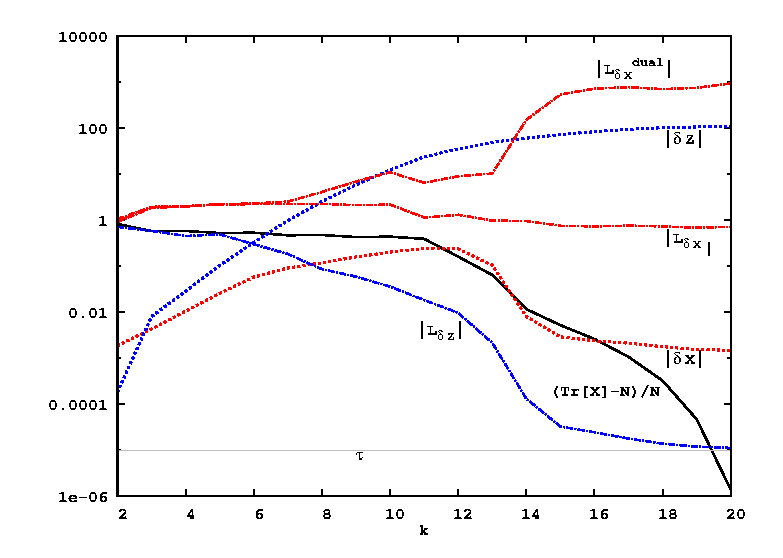
\includegraphics[width=3.5in]{8x_33_nanotube_cond10_tau-5.eps}
 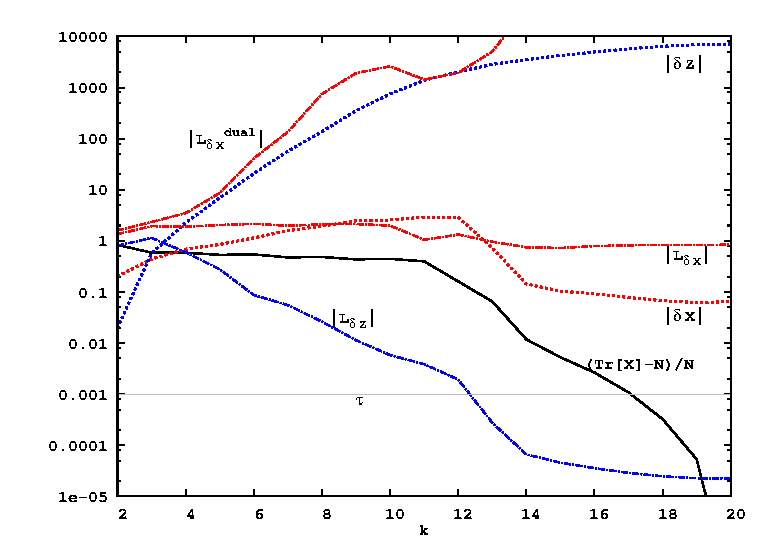
\includegraphics[width=3.5in]{8x_33_nanotube_cond10_tau-3.eps}
\end{figure}


\subsection{\bf  Analysis}


\begin{figure}[h]
  \caption{equation...}
 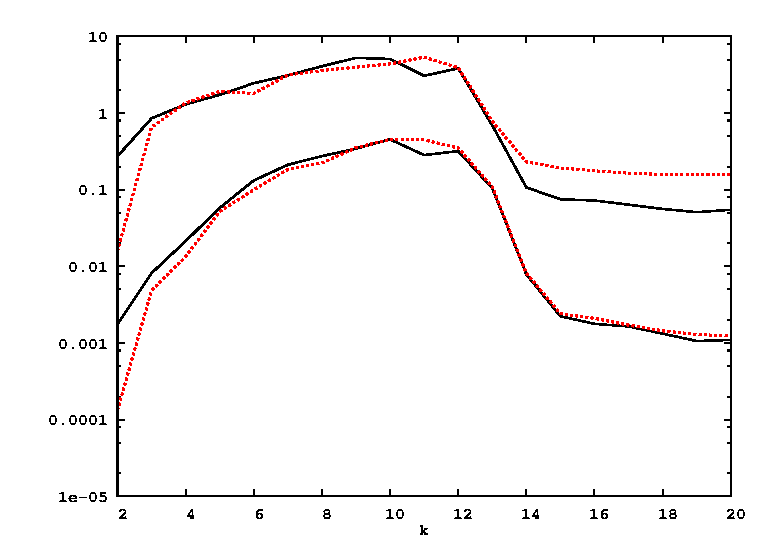
\includegraphics[width=3.5in]{8x_33_nanotube_cond10_compare_errors.eps}
\end{figure}




\begin{equation}
 \{ \widetilde{\mat{z}}^\dagger_{k} \cdot \mat{s} \cdot  \widetilde{\mat{z}}_{k-1} \} 
\rightarrow \mat{p}_+\left[\mat{s} \right]
\end{equation}


\begin{equation}
\{ \mat{s} \cdot \delta {\widehat{\mat{z}}}_{k-1}
\cdot \tt{m}\left[\mat{x}_{k-1} \right]    \} 
\rightarrow \mat{n}\left[\mat{s} \right]
\end{equation}

\begin{multline}
 \delta {\mat{z}}_{k-1} \approx \Delta^{\widetilde{\mat{z}}_{k-2} \cdot \tt{m}\left[ \widetilde{\mat{x}}_{k-2}\right]}_\tau 
+ \mat{z}_{k-2} \cdot \tt{m}'\left[ \widetilde{\mat{x}}_{k-2}\right] \cdot \delta \mat{x}_{k-2} \\
+\delta \mat{z}_{k-2} \cdot \tt{m} \left[\widetilde{\mat{x}}_{k-2} \right] 
\end{multline}

\begin{multline}
\lVert \delta {\mat{z}}_{k-1} \rVert \lesssim
\lVert \mat{z}_{k-2} \rVert \left( \;  \tau \, \lVert \tt{m} \left[\widetilde{\mat{x}}_{k-2} \right]  \rVert \right.   \\ \left.
+ \; \lVert \delta {\mat{x}}_{k-2} \rVert   \lVert \tt{m}' \left[\widetilde{\mat{x}}_{k-2} \right] \rVert \; \right)
\end{multline}

\begin{equation}
\lVert \mat{z}_{k} \rVert  \rightarrow \sqrt{\kappa\left(\mat{s} \right)}
\end{equation}

\section{Conclusion}


\paragraph{potential for data oriented  mathematics}
%%eg vs row-col picture.  Example of exact exchange w/DBSR 



\end{document}
